%!TEX root = ../doc.tex
\documentclass[../doc.tex]{subfiles}

\begin{document}
\chapter{Discontinuous Galerkin VEF Discretizations} \label{chap:dgvef}
In this chapter, we design a family of independent VEF discretizations for the linear, steady-state transport problem that can be efficiently and scalably solved with high-order accuracy, in multiple dimensions, and on curved meshes. Our approach is to begin with discretization techniques known to have effective preconditioners on the simpler case of radiation diffusion (i.e.~the model Poisson problem) and adapt them to the VEF equations. 
By using the Eddington tensor and boundary factor interpolation procedure established in \cite{two-level-independent-warsa}, these methods achieve both rapid convergence in outer fixed-point iterations and in inner linear solver iterations when paired with a high-order \gls{dg} discretization of \gls{sn} transport. 

In particular, we extend the unified analysis of DG methods developed for elliptic problems presented by \textcite{Arnold2002} to the VEF equations to derive analogs of the \gls{ip}, \gls{br2}, \gls{mdldg}, and \gls{cg} techniques.
We show that the IP and BR2 VEF methods are effectively preconditioned by the subspace correction method from \textcite{Pazner2021} and that \gls{amg} is effective for the \gls{cg} and \gls{mdldg} discretizations.
\textcite{dima_dfem} also applied DG techniques to the VEF equations but they discretize the first-order form of the VEF equations and only consider lowest-order elements in one dimension.
We note that our CG operator is equivalent to extending the continuous finite element VEF discretization in \cite{two-level-independent-warsa} to multiple dimensions, arbitrary-order, and curved meshes.

The chapter proceeds as follows. We first introduce the high-level concepts used to derive DG discretizations of the second-order form of elliptic partial differential equations. 
We then extend Arnold's unified framework to the VEF moment system. The \gls{ip}, \gls{br2}, and \gls{mdldg} methods are derived from this framework through the specification of the numerical fluxes. A discussion of the implementation of the so-called lifting operators that are used to stabilize the BR2 and MDLDG discretizations is provided.
A continuous finite element discretization is then extracted from the DG framework.  
Section \ref{dgvef_sec:subspace} discusses the \gls{usc} preconditioner and its implementation. 
We conclude with computational results.
We show that all the methods presented achieve high-order accuracy on curved meshes through the method of manufactured solutions, preserve the thick diffusion limit both on orthogonal and a severely distorted curved mesh, and are effective on the linearized, steady-state crooked pipe problem in both outer fixed-point iterations and inner preconditioned linear solver iterations.
The parallel performance of the \gls{ip} and \gls{cg} methods is demonstrated with a weak scaling study.

\section{Arnold's Unified Framework}
\textcite{Arnold2002} derive a family of DG methods for the model elliptic problem: 
	\begin{subequations}
	\begin{equation} \label{dgvef:poisson_vec}
		\vec{q} = \nabla u \,, 
	\end{equation}
	\begin{equation} \label{dgvef:poisson_sca}
		-\nabla\cdot\vec{q} = f\,,
	\end{equation}
	\end{subequations}
with Dirichlet boundary conditions. Recall that the DG finite element space $Y_p$ is defined as the space of piecewise polynomials with no continuity enforced between elements. An example of a one-dimensional member of the space $Y_1$ is shown in Fig.~\ref{dgvef:dg1d}. 
Global derivatives of functions in the DG space are not well defined due to their discontinuity along interior mesh interfaces.
We must then use integration by parts formulae applied on each element to ``offload'' derivatives away from such functions. For each element, this generates a volumetric term and a surface term. For the surface term, we must provide an additional piece of information known as the numerical flux.  
Note that, for some function $u\in Y_p$, $u|_K$ is a smooth polynomial function meaning that $u$ is \emph{locally} differentiable on each element so that $\nablah u$ is well defined. 
% --- example 1D DG element --- 
\begin{figure}
\centering
\includegraphics[width=.5\textwidth]{figs/dg1d.pdf}
\caption{An example of a one-dimensional piecewise discontinuous function that is a member of the linear DG space, $Y_1$.}
\label{dgvef:dg1d}
\end{figure}

The procedure laid forth in \textcite{Arnold2002} is to discretize and manipulate the weak form of the vector-valued equation so that the vector variable can be eliminated. This discrete elimination is then inserted into the scalar equation. 
To particularize, we discretize Eq.~\ref{dgvef:poisson_vec} in such a way that the variable $\vec{q}$ can be eliminated on each element and insert this discrete elimination into a discretization for Eq.~\ref{dgvef:poisson_sca}. 
The discretization is complete by defining suitable numerical fluxes that ensure the resulting algebraic system will be non-singular. 

These steps are demonstrated using sparsity plots in Fig.~\ref{dgvef:unified_spy}. The left diagram shows a naive discretization of the first-order form of Poisson's equation where the vector variable is approximated in such a way that it is coupled to its neighbors. This leads to the coupling shown in the $(1,1)$ block. This coupling causes the $(1,1)$ block to have a dense inverse which makes elimination of the vector variable impractical. The center diagram shows the approach of \textcite{Arnold2002}: the vector variable is approximated such that it is not coupled to its neighbors. This allows the $(1,1)$ block to be block diagonal by element. We can then eliminate the vector variable by inverting the block of degrees of freedom corresponding to each element individually. The right diagram shows the resulting system after performing this element-by-element block Gaussian elimination. The $(2,2)$ block is now dependent only on the scalar variable's degrees of freedom. By solving the global system for the scalar variable in the $(2,2)$ block, the vector variable can be computed using back substitution on each element. 
% --- depiction of unified process --- 
\begin{figure}
\centering
\begin{subfigure}{.32\textwidth}
	\centering
	\includegraphics[width=\textwidth]{figs/dgvef/unified.pdf}
	\caption{}
\end{subfigure}
\begin{subfigure}{.32\textwidth}
	\centering
	\includegraphics[width=\textwidth]{figs/dgvef/unified_1.pdf}
	\caption{}
\end{subfigure}
\begin{subfigure}{.32\textwidth}
	\centering
	\includegraphics[width=\textwidth]{figs/dgvef/unified_2.pdf}
	\caption{}
\end{subfigure}
\caption{Sparsity plots depicting DG discretizations of the Poisson equation in first-order form. The degrees of freedom are ordered so that the first block row corresponds to the vector variable and the second to the scalar variable. (a) shows a ``naive'' approach where the vector variable is coupled to its neighbor. This causes the $(1,1)$ block to be globally connected, preventing practical elimination of the vector variable. (b) shows the unified approach where the vector variable is discretized so that it can be eliminated locally on each element. (c) shows the resulting block system after performing this elimination. }
\label{dgvef:unified_spy}
\end{figure}

The present goal is to adapt this framework to the VEF equations: 
	\begin{subequations}
	\begin{equation}
		\nabla\cdot\paren{\E\varphi} + \sigma_t \vec{J} = \vec{Q}_1 \,, \quad \x \in \D\,,
	\end{equation}
	\begin{equation}
		\nabla\cdot\vec{J} + \sigma_a \varphi = Q_0 \,, \quad \x \in \D\,,
	\end{equation}
	\begin{equation}
		\vec{J}\cdot\n = E_b \varphi + 2\Jin \,, \quad \x \in \partial \D\,. 
	\end{equation}
	\end{subequations}
By extending this framework to the VEF equations, we can easily derive analogs of any of the DG methods presented in \cite{Arnold2002}. 
We will see significant differences in the final bilinear form since the Eddington tensor is inside the divergence.
Additionally, the presence of a right-hand side in the first moment equation as well as non-unit coefficients and Robin-style boundary conditions introduce further complications not discussed in \cite{Arnold2002}.

\section{Adaption of the Unified Framework to VEF} 
We seek the VEF scalar flux in the degree-$p$ DG finite element space $Y_p$ and the current in the degree-$p$ vector-valued DG finite element space $\vDG$. The weak form is then: find $(\varphi,\vec{J}) \in Y_p \times \vDG$ such that for all $K \in \meshT$: 
	\begin{subequations}
	\begin{equation}
		\int_{\partial K} \vec{v}\cdot\widehat{\E\varphi}\n_K \ud s - \int_K \nabla\vec{v} : \E \varphi \ud \x + \int_K \sigma_t \, \vec{v}\cdot\vec{J} \ud \x = \int_K \vec{v}\cdot\vec{Q}_1 \ud \x \,, \quad \forall \vec{v} \in [\mathbb{Q}_p(K)]^{\dim} \,, 
	\end{equation}
	\begin{equation}
		\int_{\partial K} u\,\widehat{\vec{J}}\cdot\n_K \ud s - \int_K \nabla u \cdot\vec{J} \ud \x + \int_K \sigma_a\, u \varphi \ud \x = \int_K u\, Q_0 \ud \x \,, \quad \forall u \in \mathbb{Q}_p(K) \,, 
	\end{equation}
	\end{subequations}
where the \emph{numerical fluxes} $\widehat{\E\varphi}$ and $\widehat{\vec{J}}$ are approximations of $\E\varphi$ and $\vec{J}$ on the boundaries of the elements in the mesh. We group the product $\E\varphi$ as the numerical flux to mimic the integration by parts of a tensor times a vector. Here, the gradient of a vector is 
	\begin{equation}
		\paren{\nabla\vec{v}}_{ij} = \paren{\pderiv{\vec{v}_i}{\x_j}} \in \R^{\dim\times \dim}
	\end{equation}
and 
	\begin{equation}
		\mat{A} : \mat{B} = \sum_{i=1}^{\dim} \sum_{j=1}^{\dim} \mat{A}_{ij} \mat{B}_{ij} \,, \quad \mat{A}, \mat{B} \in \R^{\dim\times \dim} 
	\end{equation}
is the scalar contraction of two tensors. Note that if $\E = \frac{1}{3}\I$ then 
	\begin{equation}
		\nabla\vec{v} : \E = \frac{1}{3}\nabla\cdot\vec{v} 
	\end{equation}
and the symmetric weak form for radiation diffusion is recovered. 

Summing the zeroth moment over all elements: 
	\begin{equation}
		\int_\Gamma \jump{u} \avg{\widehat{\vec{J}}\cdot\n} \ud s + \int_{\Gamma_0} \avg{u}\jump{\widehat{\vec{J}}\cdot\n} \ud s - \int \nablah u \cdot \vec{J} \ud \x + \int \sigma_a \, u\varphi \ud \x = \int u\, Q_0 \ud \x \,,
	\end{equation}
where the jumps and averages identity (Eq.~\ref{fem:jumps_avg_id}) was used. We will now use the discrete first moment to determine a functional form for $\vec{J}$. Integrating by parts locally over element $K$, we have that 
	\begin{equation} \label{dgvef:identity}
		\int_K \nabla\vec{v} : \E \varphi \ud \x = \int_{\partial K} \vec{v}\cdot\E\varphi\n_K \ud s - \int_K \vec{v}\cdot\nabla\cdot\paren{\E\varphi} \ud \x \,. 
	\end{equation}
The first moment's weak form on each element becomes: 
	\begin{equation}
		\int_{\partial K} \vec{v}\cdot\paren{\widehat{\E\varphi}\n_K - \E\varphi\n_K} \ud s + \int_K \vec{v}\cdot\nabla\cdot\paren{\E\varphi} \ud \x + \int_K \sigma_t \, \vec{v}\cdot\vec{J} \ud \x = \int_K \vec{v} \cdot\vec{Q}_1 \ud \x \,, \quad \forall \vec{v} \in [\mathbb{Q}_p(K)]^{\dim} \,. 
	\end{equation}
Summing over all elements and using the jumps and averages identity, the weak form for the first moment is:  
	\begin{multline} \label{dgvef:weak_strong}
		\int_\Gamma \avg{\vec{v}}\cdot\jump{\widehat{\E\varphi}\n - \E\varphi\n} \ud s + \int_{\Gamma_0} \jump{\vec{v}} \cdot \avg{\widehat{\E\varphi}\n - \E\varphi\n} \ud s \\+ \int \vec{v}\cdot\nablah \cdot\paren{\E\varphi} \ud \x + \int \sigma_t \, \vec{v}\cdot\vec{J} \ud \x = \int \vec{v}\cdot\vec{Q}_1 \ud \x \,, \quad \forall \vec{v} \in \vDG \,, 
	\end{multline}
where $\nablah\cdot\paren{\E\varphi}$ is evaluated as $\nablah\cdot\paren{\E\varphi} = \E\nablah \varphi + \paren{\nablah\cdot\E}\!\varphi$, and the term $\nablah\cdot\E$ is computed using Eq.~\ref{sn:Edd_div}. 

We now wish to write all terms as volumetric integrals so that a functional form for the current can be found. To that end, define \emph{lifting operators} $\vec{r}(\vec{\tau}) \in \vDG$ and $\vec{\ell}(\vec{\chi}) \in \vDG$ such that 
	\begin{subequations}
	\begin{equation} \label{dgvef:lift-r}
		\int \sigma_t\, \vec{v}\cdot\vec{r}(\vec{\tau}) \ud \x = - \int_{\Gamma} \avg{\vec{v}} \cdot \vec{\tau} \ud s \,, \quad \forall \vec{v} \in \vDG \,, 
	\end{equation}
	\begin{equation} \label{dgvef:lift-l}
		\int \sigma_t \, \vec{v}\cdot\vec{\ell}(\vec{\chi}) \ud \x = -\int_{\Gamma_0} \jump{\vec{v}} \cdot \vec{\chi} \ud s \,, \quad \forall \vec{v} \in \vDG \,, 
	\end{equation}
	\end{subequations}
where $\vec{\tau}$ and $\vec{\chi}$ are vector functions that are singled-valued on $\Gamma_0$. 
Note that the lifting operators are finite element grid functions just as the current is and that the left hand sides are simply the $\vDG$ total interaction mass matrix.
Since $\vDG$ is piecewise discontinuous, the $\vDG$ mass matrix is block-diagonal by element and thus the systems of equations corresponding to Eqs. \ref{dgvef:lift-r} and \ref{dgvef:lift-l} are amenable to efficient direct factorization. The computational aspects of lifting operators are discussed in Section \ref{dgvef_sec:lifting}. 

Setting $\vec{\tau} = \jump{\widehat{\E\varphi}\n - \E\varphi\n}$ and $\vec{\chi} = \avg{\widehat{\E\varphi}\n - \E\varphi\n}$ and using the definitions of the lifting operators, Eq.~\ref{dgvef:weak_strong} can be written entirely in terms of volumetric integrals as: 
	\begin{equation}
		\int \sigma_t\, \vec{v}\cdot\vec{J} \ud \x = \int \sigma_t\, \vec{v}\cdot\bracket{\frac{1}{\sigma_t} \paren{\vec{Q}_1 - \nablah\cdot\paren{\E\varphi}} + \vec{r}\!\paren{\jump{\widehat{\E\varphi}\n - \E\varphi\n}} + \vec{\ell}\!\paren{\avg{\widehat{\E\varphi}\n - \E\varphi\n}}} \ud \x 
	\end{equation}
for all $\vec{v}\in \vDG$. Subtracting the right hand side and setting the integrand to zero implies that 
	\begin{equation} \label{dgvef:current_form}
		\vec{J} = \frac{1}{\sigma_t}\paren{\vec{Q}_1 - \nablah\cdot\paren{\E\varphi}} + \vec{r}\!\paren{\jump{\widehat{\E\varphi}\n - \E\varphi\n}} + \vec{\ell}\!\paren{\avg{\widehat{\E\varphi}\n - \E\varphi\n}}\,. 
	\end{equation}
Observe that the above represents the element-local strong form of the current, $\frac{1}{\sigma_t}\paren{\vec{Q}_1 - \nablah\cdot\paren{\E\varphi}}$ found by analytically eliminating the current, with additional terms that capture the effect of the numerical fluxes. In other words, we have derived the \emph{discrete} elimination of the current. 

Using this discrete form for the current and the definitions of the lifting operators to convert from volumetric integrals back to surface integrals, the zeroth moment becomes: 
	\begin{multline} \label{dgvef:familynobc}
		\int_\Gamma \jump{u} \avg{\widehat{\vec{J}}\cdot\n} \ud s + \int_{\Gamma_0} \avg{u}\!\jump{\widehat{\vec{J}}\cdot\n} \ud s + \int_\Gamma \avg{\frac{\nablah u}{\sigma_t}} \cdot \jump{\widehat{\E\varphi}\n - \E\varphi\n} \ud s \\ 
		+ \int_{\Gamma_0} \jump{\frac{\nablah u}{\sigma_t}} \cdot \avg{\widehat{\E\varphi}\n - \E\varphi\n} \ud s + \int \nablah u \cdot \frac{1}{\sigma_t}\nablah\cdot\paren{\E\varphi} \ud \x + \int \sigma_a\, u \varphi \ud \x \\ 
		= \int u\, Q_0 \ud \x + \int \nablah u \cdot \frac{\vec{Q}_1}{\sigma_t} \ud \x \,, \quad \forall u \in Y_p \,. 
	\end{multline}
On boundary faces, we apply the Miften-Larsen boundary conditions by setting 
	\begin{equation} \label{dgvef:ml_bdr_flux}
		\widehat{\vec{J}}\cdot\n = E_b \varphi + 2\Jin \,, \quad \widehat{\E\varphi}\n = \E\varphi\n \,, \quad \text{on} \ \mathcal{F} \in \Gamma_b \,. 
	\end{equation}
% All the methods we consider use 
% 	\begin{equation} \label{dgvef:num_scalar_flux}
% 		\widehat{\E\varphi}\n = \avg{\E\varphi\n} \,, \quad \text{on} \ \mathcal{F} \in \Gamma \,, 
% 	\end{equation}
% where on a boundary face $\avg{\E\varphi\n} = \E\varphi\n$ from the definition of the average on a boundary face. In this way, the second condition of the Miften-Larsen boundary condition is encompassed in this definition. Using this numerical flux, we have that 
% 	\begin{subequations}
% 	\begin{equation}
% 		\jump{\widehat{\E\varphi}\n - \E\varphi\n} = \begin{cases}
% 			-\jump{\E\varphi\n} \,, & \mathcal{F} \in \Gamma_0 \\ 
% 			0 \,, & \mathcal{F} \in \Gamma_b 
% 		\end{cases} \,,
% 	\end{equation}
% 	\begin{equation}
% 		\avg{\widehat{\E\varphi}\n - \E\varphi\n} = 0 \,, \quad \forall \mathcal{F} \in \Gamma \,. 
% 	\end{equation}
% 	\end{subequations}
All the methods we consider use so-called conservative numerical fluxes such that 
	\begin{subequations}
	\begin{equation}
		\jump{\widehat{\vec{J}}\cdot\n} = 0 \,, \quad \avg{\widehat{\vec{J}}\cdot\n} = \widehat{\vec{J}}\cdot\n \,, \quad \text{on} \ \mathcal{F} \in \Gamma_0 \,, 
	\end{equation}
	\begin{equation}
		\jump{\widehat{\E\varphi}\n} = 0 \,, \quad \avg{\widehat{\E\varphi}\n} = \widehat{\E\varphi}\n \,, \quad \text{on} \ \mathcal{F} \in \Gamma_0 \,. 
	\end{equation}
	\end{subequations}
Using the boundary conditions and the assumption of conservative numerical fluxes, Eq.~\ref{dgvef:familynobc} becomes: 
	\begin{multline} \label{dgvef:family}
		\int_{\Gamma_b} E_b\, u \varphi \ud s + \int_{\Gamma_0} \jump{u} \widehat{\vec{J}}\cdot\n \ud s - \int_{\Gamma_0} \avg{\frac{\nablah u}{\sigma_t}} \cdot \jump{\E\varphi\n} \ud s \\+ \int_{\Gamma_0} \jump{\frac{\nablah u}{\sigma_t}} \cdot \avg{\widehat{\E\varphi}\n - \E\varphi\n} \ud s + \int \nablah u \cdot \frac{1}{\sigma_t}\nablah\cdot\paren{\E\varphi} \ud \x + \int \sigma_a\, u \varphi \ud \x \\ 
		= \int u\, Q_0 \ud \x + \int \nablah u \cdot \frac{\vec{Q}_1}{\sigma_t} \ud \x - 2\int_{\Gamma_b} u\, \Jin \ud s \,, \quad \forall u \in Y_p \,. 
	\end{multline}
Equation \ref{dgvef:family} defines a \emph{family} of DG methods. That is, through the specification of the numerical fluxes on interior faces, analogs of all the methods listed in \cite{Arnold2002} can be derived.

\section{Specification of Numerical Fluxes}
All the methods we consider use numerical fluxes of the form 
	\begin{subequations}
	\begin{equation}
		\widehat{\vec{J}}\cdot\n = \avg{\frac{1}{\sigma_t}\paren{\vec{Q}_1 - \nablah\cdot\paren{\E\varphi}}\cdot\n} + \alpha(\varphi) \,, \quad \text{on} \ \Gamma_0 \,, 
	\end{equation}
	\begin{equation}
		\widehat{\E\varphi}\n = \avg{\E\varphi\n} + \vec{\theta}(\varphi) \,,\quad \text{on} \ \Gamma_0 \,, 
	\end{equation}
	\end{subequations}
where $\alpha(\varphi)$ and $\vec{\theta}(\varphi)$ are single-valued functions whose purpose is to ensure a stable discretization.
The \gls{ip}, \gls{br2}, and \gls{ldg} methods differ only in the choice of $\alpha(\varphi)$ and $\vec{\theta}(\varphi)$. With these numerical fluxes, Eq.~\ref{dgvef:family} becomes: 
	\begin{multline} \label{dgvef:family_alpha}
		\int_{\Gamma_b} E_b\, u \varphi \ud s + \int_{\Gamma_0} \jump{u} \alpha(\varphi) \ud s - \int_{\Gamma_0} \jump{u} \avg{\frac{1}{\sigma_t}\nablah\cdot\paren{\E\varphi}\cdot\n} \ud s - \int_{\Gamma_0} \avg{\frac{\nablah u}{\sigma_t}} \cdot \jump{\E\varphi\n} \ud s \\ + \int_{\Gamma_0} \jump{\frac{\nablah u}{\sigma_t}} \cdot \vec{\theta}(\varphi) \ud s
		+ \int \nablah u \cdot \frac{1}{\sigma_t}\nablah\cdot\paren{\E\varphi} \ud \x + \int \sigma_a\, u \varphi \ud \x \\ 
		= \int u\, Q_0 \ud \x + \int \nablah u \cdot \frac{\vec{Q}_1}{\sigma_t} \ud \x - \int_{\Gamma_0} \jump{u} \avg{\frac{\vec{Q}_1\cdot\n}{\sigma_t}} \ud s - 2\int_{\Gamma_b} u\, \Jin \ud s \,, \quad \forall u \in Y_p \,. 
	\end{multline}
Recall that this form has already applied boundary conditions according to Eq.~\ref{dgvef:ml_bdr_flux}. In other words, the above corresponds to a DG scheme with the following numerical fluxes:
		\begin{subequations}
		\begin{equation}
			\widehat{\vec{J}}\cdot\n = \begin{cases}
				\avg{\frac{1}{\sigma_t}\paren{\vec{Q}_1 - \nablah\cdot\paren{\E\varphi}}\cdot\n} + \alpha(\varphi) \,, & \text{on} \ \Gamma_0 \\ 
				E_b \varphi + 2\Jin \,, & \text{on} \ \Gamma_b 
			\end{cases} \,, 
		\end{equation}
		\begin{equation}
			\widehat{\E\varphi}\n = \begin{cases}
				\avg{\E\varphi\n} + \vec{\theta}(\varphi) \,, & \text{on} \ \Gamma_0 \\ 
				\E\varphi\n \,, & \text{on} \ \Gamma_b 
			\end{cases} \,.
		\end{equation}
		\end{subequations}

\subsection{Interior Penalty} \label{dgvef_sec:ip}
An interior penalty-like method uses 
	\begin{equation}
		\alpha(\varphi) = \kappa \jump{\varphi} \,, \quad \vec{\theta}(\varphi) = 0 \,, 
	\end{equation}
where $\kappa$ is the penalty parameter. IP methods require that $\kappa \propto \sigma_t^{-1} p^2/h$ in order to guarantee stability. The full IP weak form is then: find $\varphi \in Y_p$ such that 
	\begin{multline} \label{dgvef:ip}
		\int_{\Gamma_b} E_b\, u \varphi \ud s + \int_{\Gamma_0} \kappa \jump{u} \jump{\varphi} \ud s - \int_{\Gamma_0} \jump{u} \avg{\frac{1}{\sigma_t}\nablah\cdot\paren{\E\varphi}\cdot\n} \ud s - \int_{\Gamma_0} \avg{\frac{\nablah u}{\sigma_t}} \cdot \jump{\E\varphi\n} \ud s \\
		+ \int \nablah u \cdot \frac{1}{\sigma_t}\nablah\cdot\paren{\E\varphi} \ud \x + \int \sigma_a\, u \varphi \ud \x \\ 
		= \int u\, Q_0 \ud \x + \int \nablah u \cdot \frac{\vec{Q}_1}{\sigma_t} \ud \x - \int_{\Gamma_0} \jump{u} \avg{\frac{\vec{Q}_1\cdot\n}{\sigma_t}} \ud s - 2\int_{\Gamma_b} u\, \Jin \ud s \,, \quad \forall u \in Y_p \,. 
	\end{multline}

\subsection{The Second Method of Bassi and Rebay (BR2)}
The \gls{br2} method uses an alternative penalty term. Let $\vec{\rho}_f(\omega)\in \vDG$ be a face-local lifting operator defined by 
	\begin{equation} \label{dgvef:rhof}
		\int \vec{v}\cdot\vec{\rho}_f(\omega) \ud \x = -\int_f \avg{\vec{v} \cdot\n} \omega \ud s \,, \quad \forall \vec{v} \in \vDG\,, \quad \text{on} \ f\in \Gamma_0 \,. 
	\end{equation}
Here, $\omega$ is a scalar function that is single-valued on the interior face $f$. Note that the integration on the left hand side is over the entire domain while the right hand side is localized to a single interior face. This means the right hand side, and thus $\vec{\rho}_f(\omega)$, will be non-zero only for the degrees of freedom in elements that share the face $f$. 

A BR2-like discretization sets 
	\begin{equation}
		\alpha(\varphi) = -\eta\avg{\vec{\rho}_f(\jump{\varphi})\cdot\n} \,, \quad \text{on} \ f \in \Gamma_0 \,, \quad \vec{\theta}(\varphi) = 0 \,,
	\end{equation}
so that the relevant term is 
	\begin{equation}
	\begin{aligned}
		\int_{\Gamma_0} \jump{u} \alpha(\varphi) \ud s &= -\sum_{f\in\Gamma_0}\int_{f} \eta\,\jump{u}\!\avg{\vec{\rho}_f(\jump{u})\cdot\n} \ud s \\
		&= \sum_{f\in\Gamma_0}\int \eta\,\vec{\rho}_f(\jump{u})\cdot\vec{\rho}_f(\jump{\varphi}) \ud \x \,.
	\end{aligned}
	\end{equation}
This BR2 numerical flux avoids the need to tune the penalty parameter while still allowing element-by-element assembly (see Section \ref{dgvef_sec:lifting}). 

The BR2 DG VEF discretization is then: find $\varphi \in Y_p$ such that 
	\begin{multline} \label{dgvef:br2}
		\int_{\Gamma_b} E_b\, u \varphi \ud s - \int_{\Gamma_0} \jump{u} \avg{\frac{1}{\sigma_t}\nablah\cdot\paren{\E\varphi}\cdot\n} \ud s - \int_{\Gamma_0} \avg{\frac{\nablah u}{\sigma_t}} \cdot \jump{\E\varphi\n} \ud s \\
		+ \sum_{f\in\Gamma_0} \int \eta\, \vec{\rho}_f(\jump{u}) \cdot \vec{\rho}_f(\jump{\varphi}) \ud \x + \int \nablah u \cdot \frac{1}{\sigma_t}\nablah\cdot\paren{\E\varphi} \ud \x + \int \sigma_a\, u \varphi \ud \x \\ 
		= \int u\, Q_0 \ud \x + \int \nablah u \cdot \frac{\vec{Q}_1}{\sigma_t} \ud \x - \int_{\Gamma_0} \jump{u} \avg{\frac{\vec{Q}_1\cdot\n}{\sigma_t}} \ud s - 2\int_{\Gamma_b} u\, \Jin \ud s \,, \quad \forall u \in Y_p \,. 
	\end{multline}

\subsection{Minimal Dissipation Local Discontinuous Galerkin}
Finally, we consider the \gls{ldg} method. In general, \gls{ldg} uses the following numerical fluxes:
	\begin{subequations}
	\begin{equation}
		\widehat{\vec{J}}\cdot\n = \avg{\vec{J}\cdot\n} + \beta\jump{\vec{J}\cdot\n} + \kappa \jump{\varphi} \,,
	\end{equation}
	\begin{equation}
		\widehat{\E\varphi}\n = \avg{\E\varphi\n} - \beta\jump{\E\varphi\n} \,,
	\end{equation}
	\end{subequations}
where $\vec{J}$ is defined as the discrete elimination of the current derived in Eq.~\ref{dgvef:current_form}. The scalar parameter $\beta$ can be defined as 
	\begin{equation}
		\beta = \begin{cases}
			1/2 \,, & \vec{w}\cdot\n > 0 \\ 
			-1/2\,, & \vec{w} \cdot\n < 0 
		\end{cases} \,, \quad \mathcal{F} \in \Gamma_0 \,,
		% \beta = \frac{1}{2}\sign(\vec{w}\cdot\n) \,, 
	\end{equation}
where $\vec{w}$ is any constant, non-zero vector. This choice imposes an arbitrary upwinding on the current that is balanced by an opposing choice for the scalar flux.
With this choice of $\beta$, the \gls{ldg} method is stable for any $\kappa \geq 0$; if $\kappa\equiv 0$, the method is referred to as the minimal dissipation \gls{ldg} method \cite{10.1007/s10915-007-9130-3}.
Using the numerical flux for the scalar flux, the discrete current simplifies to 
	\begin{equation}
		\vec{J} = \frac{1}{\sigma_t}\paren{\vec{Q}_1 - \nablah \cdot\paren{\E\varphi}} - \vec{r}_0\!\paren{\jump{\E\varphi\n}} - \vec{\ell}\!\paren{\beta\jump{\E\varphi\n}} \,,
	\end{equation}
where $\vec{r}_0(\vec{\tau}) \in \vDG$ is another lifting operator defined by 
	\begin{equation}
	 	\int \sigma_t\, \vec{v}\cdot\vec{r}_0(\vec{\tau}) \ud \x = -\int_{\Gamma_0} \avg{\vec{v}}\cdot \vec{\tau} \ud s \,, \quad \forall \vec{v} \in \vDG \,, 
	\end{equation} 
that differs from $\vec{r}(\vec{\tau})$ only in the region of integration on the right hand side. The \gls{ldg} method is then equivalent to setting 
	\begin{subequations}
	\begin{multline}
		\alpha(\varphi) = -\avg{\vec{r}_0\!\paren{\jump{\E\varphi\n}}\cdot\n + \vec{\ell}\!\paren{\beta\jump{\E\varphi\n}}\cdot\n} \\+ \beta\jump{\frac{1}{\sigma_t}\paren{\vec{Q}_1 - \nablah\cdot\paren{\E\varphi}}\cdot\n - \vec{r}_0\!\paren{\jump{\E\varphi\n}}\cdot\n - \vec{\ell}\!\paren{\beta\jump{\E\varphi\n}}\cdot\n} + \kappa\jump{\varphi} \,,
	\end{multline}
	\begin{equation}
		\vec{\theta}(\varphi) = -\beta\jump{\E\varphi\n} \,.
	\end{equation}
	\end{subequations}
We then have that 
	\begin{multline}
		\int_{\Gamma_0} \jump{u} \alpha(\varphi) \ud s = \int_{\Gamma_0} \beta \jump{u}\jump{\frac{\vec{Q}_1\cdot\n}{\sigma_t}} \ud s - \int_{\Gamma_0}\beta\jump{u}\jump{\frac{1}{\sigma_t}\nablah\cdot\paren{\E\varphi}\cdot\n} \ud s \\
		+ \int \paren{\vec{\rho}_0\!\paren{\jump{u}} + \vec{\lambda}\!\paren{\beta\jump{u}}}\cdot\paren{\vec{r}_0\!\paren{\jump{\E\varphi\n}} + \vec{\ell}\!\paren{\beta\jump{\E\varphi\n}}} \ud \x + \int_{\Gamma_0} \kappa \jump{u}\jump{\varphi} \ud s 
	\end{multline}
where $\vec{\rho}_0(\omega), \vec{\lambda}(\upsilon) \in \vDG$ such that 
	\begin{equation}
		\int \vec{v} \cdot \vec{\rho}_0(\omega) \ud \x = -\int_{\Gamma_0} \avg{\vec{v}\cdot\n} \omega \ud s \,, \quad \forall \vec{v} \in \vDG \,,
	\end{equation}
	\begin{equation}
		\int \vec{v} \cdot \vec{\lambda}(\upsilon) \ud \x = -\int_{\Gamma_0} \jump{\vec{v}\cdot\n} \upsilon \ud s \,, \quad \forall \vec{v} \in \vDG \,, 
	\end{equation}
are analogs of $\vec{r}_0(\vec{\tau})$ and $\vec{\ell}(\vec{\chi})$, respectively, that do not include the total interaction cross section in the left hand side mass matrices and have scalar arguments. The \gls{ldg} VEF discretization is then: find $\varphi \in Y_p$ such that 
	\begin{multline} \label{dgvef:ldg}
		\int_{\Gamma_b} E_b\, u \varphi \ud s + \int_{\Gamma_0} \kappa\, \jump{u}\jump{\varphi} \ud s - \int_{\Gamma_0} \jump{u} \avg{\frac{1}{\sigma_t}\nablah\cdot\paren{\E\varphi}\cdot\n} \ud s - \int_{\Gamma_0} \avg{\frac{\nablah u}{\sigma_t}} \cdot \jump{\E\varphi\n} \ud s \\
		+ \int \paren{\vec{\rho}_0\!\paren{\jump{u}} + \vec{\lambda}\!\paren{\beta\jump{u}}}\cdot\paren{\vec{r}_0\!\paren{\jump{\E\varphi\n}} + \vec{\ell}\!\paren{\beta\jump{\E\varphi\n}}} \ud \x \\+ \int \nablah u \cdot \frac{1}{\sigma_t}\nablah\cdot\paren{\E\varphi} \ud \x + \int \sigma_a\, u \varphi \ud \x 
		\\= \int u\, Q_0 \ud \x + \int \nablah u \cdot \frac{\vec{Q}_1}{\sigma_t} \ud \x - \int_{\Gamma_0} \jump{u} \paren{\avg{\frac{\vec{Q}_1\cdot\n}{\sigma_t}} + \beta\jump{\frac{\vec{Q}_1\cdot\n}{\sigma_t}}} \ud s - 2\int_{\Gamma_b} u\, \Jin \ud s \,, \quad \forall u \in Y_p \,. 
	\end{multline}
The advantage of \gls{ldg} is that the penalty parameter does not need to scale with the mesh size. However, the \gls{ldg} stabilization term has a non-compact stencil that connects neighbors of neighbors, leading to less sparsity than the IP or BR2 methods. 

\section{Implementation of Lifting Operators} \label{dgvef_sec:lifting}
Consider the face-local lifting operator $\vec{\rho}_f(\omega)$ used in the BR2 stabilization term defined in Eq.~\ref{dgvef:rhof} with $\omega = \jump{u}$ which satisfies
	\begin{equation} \label{eq:lift_particularize}
		\int \vec{v}\cdot\vec{\rho}_f(\jump{u}) \ud \x = -\int_{f} \avg{\vec{v}\cdot\n} \jump{u} \ud s \,, \quad \forall \vec{v} \in \vDG\,, \quad \text{on} \ f \in \Gamma_0 \,. 
	\end{equation}
Let $\ubar{y}$ represent the vector of degrees of freedom corresponding to a $Y_p$ or $\vDG$ grid function $y$. Let $\vec{v},\vec{w} \in \vDG$ and define 
	\begin{equation}
		\ubar{v}^T \mat{M} \ubar{w} = \int \vec{v}\cdot\vec{w} \ud \x 
	\end{equation}
as the $\vDG$ mass matrix. Further, define 
	\begin{equation}
		\ubar{v}^T \mat{A}_f \ubar{u} = - \int_f \avg{\vec{v}\cdot\n} \jump{u} \ud s \,, \quad \text{on} \ f \in \Gamma_0 \,, 
	\end{equation}
for $u \in Y_p$. 
Equation \ref{eq:lift_particularize} is then equivalent to 
	\begin{equation}
		\mat{M} \ubar{\rho}_f(\jump{u}) = \mat{A}_f \ubar{u} \iff \ubar{\rho}_f(\jump{u}) = \mat{M}^{-1} \mat{A}_f \ubar{u} \,. 
	\end{equation}
Since the $\vDG$ mass matrix is block diagonal by element, its inverse can be computed and stored without fill-in by simply inverting each block individually. The BR2 stabilization term can then be written as 
	\begin{equation}
	\begin{aligned}
		\sum_{f\in\Gamma_0}\int \vec{\rho}_f(\jump{u}) \cdot\vec{\rho}_f(\jump{\varphi}) \ud \x &= \sum_{f\in\Gamma_0}\ubar{\rho}_f(\jump{u})^T \mat{M} \ubar{\rho}_f(\jump{\varphi}) \\
		&= \sum_{f\in\Gamma_0}\ubar{u}^T \mat{A}_f^T \mat{M}^{-T} \mat{M} \mat{M}^{-1} \mat{A}_f \ubar{\varphi} \\
		&= \sum_{f\in\Gamma_0}\ubar{u}^T \mat{A}_f^T \mat{M}^{-1} \mat{A}_f \ubar{\varphi} 
	\end{aligned}
	\end{equation}
since $\mat{M}$ is symmetric. Again, since $\mat{M}^{-1}$ is block diagonal by element and the products $\mat{A}_f\ubar{\varphi}$ and $\ubar{u}^T \mat{A}_f^T$ are non-zero only on degrees of freedom that share the face $f$, each argument of the sum only contributes to the degrees of freedom that share the face $f$. Due to this, the matrix $\sum_{f\in\Gamma_0} \mat{A}_f^T \mat{M}^{-1} \mat{A}_f$ can be assembled face by face. 

Next, consider one part of the LDG stabilization term: 
	\begin{equation}
		\int \vec{\rho}_0(\jump{u}) \cdot \vec{r}_0(\jump{\E\varphi\n}) \ud \x \,. 
	\end{equation}
Let, 
	\begin{equation}
		\ubar{v}^T \mat{B} \ubar{\varphi} = -\int_{\Gamma_0} \avg{\vec{v}}\cdot \jump{\E\varphi\n} \ud s \,,
	\end{equation}
and further define the total interaction $\vDG$ mass matrix as 
	\begin{equation}
		\ubar{v}^T \mat{M}_t \ubar{w} = \int \sigma_t\, \vec{v} \cdot \vec{w} \ud \x \,, 
	\end{equation}
so that $\ubar{r}_0\!\paren{\jump{\E\varphi\n}} = \mat{M}_t^{-1} \mat{B} \ubar{\varphi}$. In addition, define 
	\begin{equation}
		\ubar{v}^T \mat{A} \ubar{u} = - \int_{\Gamma_0} \avg{\vec{v}\cdot\n} \jump{u} \ud s \,, 
	\end{equation}
such that $\mat{A} = \sum_{f\in\Gamma_0} \mat{A}_f$. The LDG stabilization term under consideration is then 
	\begin{equation}
	\begin{aligned}
	 	\int \vec{\rho}_0(\jump{u})\cdot\vec{r}_0\!\paren{\jump{\E\varphi\n}} \ud \x &= \ubar{\rho}_0(\jump{u})^T \mat{M} \ubar{r}_0\!\paren{\jump{\E\varphi\n}} \\
		&= \ubar{u}^T \mat{A}^T \mat{M}^{-T} \mat{M} \mat{M}_t^{-1} \mat{B} \ubar{\varphi} \\
		&= \ubar{u}^T \mat{A}^T\mat{M}_t^{-1}\mat{B} \ubar{\varphi} \,.
	\end{aligned}
	\end{equation} 
Note that since the matrices $\mat{A}$ and $\mat{B}$ are not face-local, this term cannot be assembled locally. The LDG stabilization term is instead formed through matrix multiplication as $\mat{A}^T\mat{M}_t^{-1}\mat{B}$. 

\section{Extracting a Continuous Discretization from the DG Framework} \label{dgvef_sec:cfem}
We now show how a \gls{cg} discretization of the VEF drift-diffusion equation can be extracted from the DG framework presented above. An approximate inversion of this operator is one stage of the subspace correction preconditioner described in Section \ref{dgvef_sec:subspace} that is used to efficiently solve the IP and BR2 VEF discretizations. This CG operator is also a VEF method itself and represents an extension to multiple dimensions, arbitrary-order, and curved meshes of the algorithm in \cite{two-level-independent-warsa}. A CG VEF method has fewer unknowns than an analogous DG method and requires simpler methods to solve the resulting linear system. We will show that this CG discretization has similar accuracy to DG and does not degrade convergence of the fixed-point iteration even in the asymptotic thick diffusion limit. However, it is unclear if using a continuous finite element space would negatively impact robustness and stability in the larger radiation-hydrodynamics multiphysics setting. 

Let $u,\varphi \in V_p$, the degree-$p$ continuous finite element space, then 
	\begin{equation}
		\jump{u} = 0 \,, \quad \jump{\varphi} = 0 \,, \quad \text{on} \ \mathcal{F}\in\Gamma_0 \,. 
	\end{equation}
However, since the Eddington tensor is still discontinuous, we have that 
	\begin{equation}
		\jump{\E\varphi\n} = \jump{\E\n} \varphi \,. 
	\end{equation}
Note that, for $u\in V_p$, $\nabla u \in \vDG$. In other words, while $u\in V_p$ is continuous $\nabla u$ is not. Thus, by starting from the DG VEF discretization and assembling onto $V_p$, we arrive at a CG VEF discretization of the form: find $\varphi \in V_p$ such that 
	\begin{multline} \label{dgvef:cg}
		\int_{\Gamma_b} E_b\, u \varphi \ud s - \int_{\Gamma_0} \avg{\frac{\nabla u}{\sigma_t}} \cdot \jump{\E\n}\!\varphi \ud s 
		+ \int \nabla u \cdot \frac{1}{\sigma_t}\nablah\cdot\paren{\E\varphi} \ud \x + \int \sigma_a\, u \varphi \ud \x \\ 
		= \int u\, Q_0 \ud \x + \int \nabla u \cdot \frac{\vec{Q}_1}{\sigma_t} \ud \x - 2\int_{\Gamma_b} u\, \Jin \ud s \,, \quad \forall u \in V_p \,. 
	\end{multline}
Observe that in the thick diffusion limit, where $\E = \frac{1}{3}\I$ and $E_b = 1/2$, a CG discretization of radiation diffusion with Marshak boundary conditions arises since $\jump{\E\n} = 0$ and $\frac{1}{\sigma_t}\nablah\cdot\paren{\E\varphi} = \frac{1}{3\sigma_t}\nabla \varphi$. 

\section{Uniform Subspace Correction Preconditioner} \label{dgvef_sec:subspace}
\textcite{Pazner2021} presents a preconditioning strategy for DG discretizations of elliptic problems based on a decomposition of the DG space. The decomposition is chosen so that the resulting preconditioner can leverage the efficiency and scalability of \gls{amg} applied to a continuous finite element discretization of an elliptic problem. The resulting scheme is closely related to preconditioning a DG operator with a CG operator. However, this method includes an additional step where a classical smoother is applied to a DG operator in order to provide a preconditioner that scales optimally with respect to the mesh size, polynomial order, and penalty parameter. Here, we present the implementation details in applying this preconditioner to the DG discretizations developed in this chapter. 

\subsection{Decomposition of the DG Space}
The DG space is split into a continuous finite element part and a discontinuous finite element part. In order to allow definition of a continuous finite element space, we restrict to the case where the DG space uses the closed Gauss-Lobatto basis on each element. Let $V_C$ denote the continuous subspace of $Y_p$. In other words, $V_C = Y_p \cap H^1(\D)$. Due to the use of Gauss-Lobatto nodes, $V_C = V_p$, the degree-$p$ continuous finite element space. 

We now seek to construct a space, $V_B$, such that $Y_p = V_C + V_B$. Here, the ``B'' subscript stands for ``boundary.'' Let $\mathcal{B}(K)$ denote the set of nodes located on the boundary of the element, $\partial K$, and $\mathcal{I}(K)$ the set of nodes located on the interior of the element. The space $V_B$ consists of functions $v_b$ such that $v_b(\vec{\x}_{K,i}) = 0$ for each $\vec{\x}_{K,i} \in \mathcal{I}(K)$ for all elements $K \in \meshT$. In other words, $v_b \in V_B$ attains a value of zero at each interior node of every element in the mesh. 
Alternatively, a function $u \in Y_p$ could be represented as $u = u_c + u_b$ where $u_c \in V_C$ and $u_b \in Y_p$. However, $V_B$ is preferred due to its smaller dimension. 

This decomposition is depicted in Fig.~\ref{dgvef:usc_fes} for the space $Y_3$. The nodes $\vec{\xi}_i \in \mathcal{B}(K)$ of $Y_3$ and $V_B$ are offset toward the interior of the element in order to show the presence of multiple nodes on each interior face in the mesh. Here, the continuous space $V_C$ is equivalent to $V_3$ the cubic continuous finite element space. The right diagram depicts the boundary space $V_B$ which has only the nodes of $Y_3$ corresponding to $\mathcal{B}(K)$ for each $K \in \meshT$. Note that $V_B$ has nodes on both sides of each interior interface. 
% --- example of decomposed FES --- 
\begin{figure}
\centering
\includegraphics[width=.85\textwidth]{figs/usc_proj.pdf}
\caption{A depiction of the degrees of freedom associated with the decomposition of the DG space. The left diagram shows the discontinuous space $Y_3$ where the nodal basis for each element interpolates through the Gauss-Lobatto points. The nodes on the boundary of each element are offset inwards in order to show the placement of nodes on both sides of the interface between interior elements. The middle diagram shows the node placement for the corresponding continuous finite element space. Here, the nodes are shared between neighboring elements. The right diagram depicts the boundary space consisting of only the nodes on the boundary of each element. }
\label{dgvef:usc_fes}
\end{figure}

We now present operators $\mat{Q} : Y_p \rightarrow V_C$ and $\mat{B} : Y_p \rightarrow V_B$ that take functions in $Y_p$ and convert them to $V_C$ and $V_B$, respectively. Let $u \in Y_p$ be given. The interpolation operator $\mat{Q}u$ copies the degrees of freedom corresponding to nodes interior to each element or on the boundary of the domain (e.g.~$\x_i \in \mathcal{I}(K)$ for each $K$ or $\x_i \in \partial\D$) so that $\mat{Q}u(\x_i) = u(\x_i)$ at each $\x_i \in \mathcal{I}(K)$ for each $K$ or $\x_i \in \partial\D$. For nodes located on interior faces of the mesh, $\mat{Q}u$ averages the values of $u$ in the elements that share the face. That is for a face $\Gamma_0 \ni \mathcal{F} = K_1 \cap K_2$, we set 
	\begin{equation}
		\mat{Q}u(\x_i) = \frac{1}{2}\paren{u|_{K_1} + u|_{K_2}} \,,
	\end{equation}
for each node $\x_i \in \mathcal{F}$. 
The action of the operator $\mat{B}$ on $u\in Y_p$ restricts $u$ to the space $V_B$. That is, degrees of freedom associated with $\mathcal{I}(K)$ for each $K$ are removed leaving only the nodes corresponding to $\mathcal{B}(K)$ for each $K$. The handling of the complications arising in $hp$ refinement (e.g.~non-conforming hanging nodes) is presented in \cite{Pazner2021}. 

\subsection{Additive Schwarz Preconditioner}
We now define a preconditioner built on the decomposition $Y_p = V_C + V_B$. Let $\mathcal{A} : Y_p \times Y_p \rightarrow \R$ denote one of the DG VEF bilinear forms derived in this chapter. We also define the linear operator $\mat{A} : Y_p \rightarrow Y_p$ such that 
	\begin{equation}
		\ubar{v}^T \mat{A} \ubar{u} = \mathcal{A}(v,u) \,, \quad u,v \in Y_p \,. 
	\end{equation}
In other words, $\mathcal{A}$ is a DG VEF bilinear form (e.g.~Eq.~\ref{dgvef:ip}) while $\mat{A}$ is the corresponding matrix. Further, we define the restrictions of $\mat{A}$ to $V_C$ and $V_B$ as 
	\begin{subequations}
	\begin{equation}
		\ubar{v}_c^T \mat{A}_c \ubar{u}_c = \mathcal{A}(v_c,u_c) \,, \quad u_c,v_c \in V_c \,,
	\end{equation}
	\begin{equation}
		\ubar{v}_b^T \mat{A}_b \ubar{u}_b = \mathcal{A}(v_b, u_b) \,, \quad u_b,v_b \in V_B \,. 
	\end{equation}
	\end{subequations}
Note that the restriction of $\mathcal{A}$ to $V_C$ represented by $\mat{A}_c$ is exactly the matrix corresponding to the CG VEF operator in Eq.~\ref{dgvef:cg}. We define the so-called \emph{elliptic projections} onto the spaces $V_C$ and $V_B$ as $\mat{P}_c : Y_p \rightarrow V_C$ and $\mat{P}_b : Y_p \rightarrow V_B$, respectively, which satisfy 
	\begin{subequations}
	\begin{equation}
		\mat{A}_c \mat{P}_c = \mat{Q} \mat{A} \,,  
	\end{equation}
	\begin{equation}
		\mat{A}_b \mat{P}_b = \mat{B} \mat{A} \,. 
	\end{equation}
	\end{subequations}
Applying the inverse, the projections are given by 
	\begin{equation}
		\mat{P}_c = \mat{A}_c^{-1} \mat{Q} \mat{A} \,,
	\end{equation}
	\begin{equation}
		\mat{P}_b = \mat{A}_b^{-1} \mat{B} \mat{A} \,. 
	\end{equation}
The spaces $V_C$ and $V_B$ are sufficiently large that $\mat{A}_c$ and $\mat{A}_b$ are impractical to invert directly. We thus approximate the inverses using $\mat{R}_c \approx \mat{A}_c^{-1}$ and $\mat{R}_b \approx \mat{A}_b^{-1}$. We use one \gls{amg} V-cycle for $\mat{R}_c$ and one iteration of point Jacobi for $\mat{R}_b$. 
The projections are prolonged to the space $Y_p$ using the transpose of their associated restriction operators. 
The preconditioned operator is given by the sum of the prolonged, approximate elliptic projections: 
	\begin{equation}
		\mat{P}^{-1}\mat{A} = (\mat{Q}^T \mat{P}_c + \mat{B}^T\mat{P}_b)\mat{A} = (\mat{Q}^T\mat{R}_c \mat{Q} + \mat{B}^T \mat{R}_b \mat{B})\mat{A} \,. 
	\end{equation}
The preconditioner $\mat{P}^{-1}$ is then 
	\begin{equation}
		\mat{P} = \mat{Q}^T\mat{R}_c \mat{Q} + \mat{B}^T \mat{R}_b \mat{B} \,. 
	\end{equation}
It is applied in two stages corresponding to $V_C$ and $V_B$ each of which include restriction to the subspace, approximately inverting the operator derived by restricting $\mat{A}$ to the subspace, and prolonging back to the original space $Y_p$. 
In \textcite{Pazner2021}, it is shown that the preconditioned system $\mat{P}^{-1}\mat{A}$ has condition number independent of the mesh size, polynomial order, and penalty parameter (if applicable). 

In the implementation, the operator $\mat{A}_c$ is computed by \emph{assembling} $\mat{A}$ onto the space $V_C$. This is an algebraic process that allows the CG operator to be formed without re-discretizing and re-evaluating the bilinear forms that comprise $\mat{A}$. This process is depicted in Fig.~\ref{dgvef:usc_assembly}. The operators $\mat{Q}$ and $\mat{B}$ are implemented in a matrix-free fashion. That is, we define only their action and transpose action onto the residual vector. Finally, the operator $\mat{R}_b$ is computed by assembling the diagonal of $\mat{A}$ and applying $\mat{B}$ so that only the degrees of freedom corresponding to $V_B$ remain. The action of $\mat{R}_b$ onto a vector $\ubar{r}$ is then equivalent to dividing the entries of $\ubar{r}$ corresponding to $\mathcal{B}(K)$ for each $K$ by the associated diagonal entry of $\mat{A}$.
% --- assembly diagram --- 
\begin{figure}
\centering
\includegraphics[width=.65\textwidth]{figs/usc_assembly.pdf}
\caption{A depiction of the assembly operator applied to the space $Y_1$ to yield an operator defined on the continuous finite element space $V_1$. By assembling a DG discretization of the VEF equations onto a suitable CG space, the CG operator can be computed without re-discretizing.}
\label{dgvef:usc_assembly}
\end{figure}

\section{Results}
The VEF algorithms described in this chapter were implemented using the MFEM \cite{MFEM,mfem-web} finite element framework. The \gls{bicg} and Jacobi solvers from MFEM were used to solve the VEF discretizations along with BoomerAMG, the AMG solver from the sparse linear algebra library \emph{hypre} \cite{hypre}. KINSOL, from the Sundials package \cite{hindmarsh2005sundials}, provided the Anderson-accelerated fixed-point solver. When iterative solver results are not presented, the parallel implementation of the sparse direct solver SuperLU \cite{lidemmel03} was used. We use the high-order DG \gls{sn} transport solver from \cite{graph_sweeps}.

Unless otherwise specified, we set the penalty parameter to 
	\begin{equation}
		\kappa_e = \avg{\frac{(p+1)^2}{\sigma_t h_e}} 
	\end{equation}
and the BR2 stabilization parameter to $\eta = 4$. We use the MDLDG method, the variant of the LDG method where $\kappa \equiv 0$ and set the upwinding vector $\vec{w}$ to be a unit vector at a $45^\circ$ angle from the $x$-axis. The VEF discretizations all use the element-local basis defined using the Gauss-Lobatto points to enable the use of the subspace correction preconditioner where required. The transport discretization is always solved with the same finite element order as the VEF scalar flux. However, we use the positive Bernstein basis \cite{doi:10.1137/11082539X} for the transport discretization. 

\subsection{Method of Manufactured Solutions}
The accuracy of the methods are determined with the \gls{mms}. The solution is set to 
	\begin{equation} \label{dgvef:mms_psi}
		\psi = \frac{1}{4\pi}\bracket{\alpha(\x) + \Omegahat\cdot\vec{\beta}(\x) + \Omegahat\otimes\Omegahat : \mat{\Theta}(\x)} \,,
	\end{equation}
where 
	\begin{subequations}
	\begin{equation}
		\alpha(\x) = \sin(\pi x) \sin(\pi y) + \delta \,, 
	\end{equation}
	\begin{equation}
		\vec{\beta}(\x) = \begin{bmatrix} 
			\sin\!\paren{\frac{2\pi(x+\omega)}{1+2\omega}}\sin\!\paren{\frac{2\pi(y+\omega)}{1+2\omega}}\\
			\sin\!\paren{\frac{2\pi(x+\omega)}{1+2\omega}}\sin\!\paren{\frac{2\pi(y+\omega)}{1+2\omega}}
		\end{bmatrix} \,,
	\end{equation}
	\begin{equation} \label{dgvef:mmsH}
		\mat{\Theta}(\x) = \begin{bmatrix} 
			\frac{1}{2}\sin\!\paren{\frac{3\pi(x+\zeta)}{1 + 2\zeta}}\sin\!\paren{\frac{3\pi(y+\zeta)}{1+2\zeta}}
			& \sin\!\paren{\frac{2\pi(x+\omega)}{1+2\omega}}\sin\!\paren{\frac{2\pi(y+\omega)}{1+2\omega}}\\
			\sin\!\paren{\frac{2\pi(x+\omega)}{1+2\omega}}\sin\!\paren{\frac{2\pi(y+\omega)}{1+2\omega}}
			& \frac{1}{4}\sin\!\paren{\frac{3\pi(x+\zeta)}{1 + 2\zeta}}\sin\!\paren{\frac{3\pi(y+\zeta)}{1+2\zeta}}
		\end{bmatrix} \,.
	\end{equation}
	\end{subequations}
The parameter $\delta = 1.25$ is used to ensure $\psi>0$ and $\zeta = 0.1$ and $\omega = 0.05$ are used to test spatially-dependent, non-isotropic inflow boundary conditions. The domain is $\D = [0,1]^2$. 
With this definition: 
	\begin{subequations}
	\begin{equation}
		\phi(\x) = \alpha(\x) + \frac{1}{3}\tr\mat{\Theta}(\x) \,,
	\end{equation}
	\begin{equation}
		\vec{J}(\x) = \frac{1}{3}\vec{\beta}(\x) \,,
	\end{equation}
	\begin{equation}
		\P(\x) = \frac{\alpha(\x)}{3}\I + \frac{1}{15}\begin{bmatrix} 
			3 \Theta_{11}(\x) + \Theta_{22}(\x) & \Theta_{12}(\x) \\ \Theta_{21}(\x) & \Theta_{11}(\x) + 3 \Theta_{22}(\x) 
		\end{bmatrix} \,. 
	\end{equation}
	\end{subequations}
This leads to an exact Eddington tensor $\E = \P/\phi$ that is dense and spatially varying. The MMS $\psi$ and $\phi$ are substituted into the transport equation to solve for the MMS source $q$ that forces the solution to Eq.~\ref{dgvef:mms_psi}. 

The accuracy of the VEF discretizations can be investigated in isolation by computing the VEF data from the MMS angular flux and setting the sources $Q_0$ and $\vec{Q}_1$ to the moments of the transport MMS source. This is accomplished by computing the VEF data from the MMS angular flux projected onto a finite element space of equal order to the VEF finite element space. An open, Gauss-Legendre basis is used for the angular flux so that the Eddington tensor will have discontinuities of magnitude $\mathcal{O}(h^{p+1})$ on interior mesh faces. The VEF data and source moments are computed using level symmetric $S_4$ angular quadrature. The VEF equations are then solved as if $\E$, $E_b$, $Q_0$, $\vec{Q}_1$, and $\Jin$ are provided data. 

We use refinements of a third-order curved mesh created by distorting an orthogonal mesh according to the velocity field of the Taylor Green vortex. This mesh distortion is generated by advecting the mesh control points with 
	\begin{equation}
		\x = \int_0^T \mat{v} \ud t \,,
	\end{equation}
where the final time $T = 0.3 \pi$ and 
	\begin{equation}
		\mat{v} = \begin{bmatrix} 
			\sin(x_1) \cos(x_2) \\
			-\cos(x_1)\sin(x_2) 
		\end{bmatrix}
	\end{equation}
is the analytic solution of the Taylor Green vortex. The time integration is calculated with 300 forward Euler time steps. An example mesh is shown in Fig.~\ref{dgvef:tgmesh}. 

% --- plot of taylor green mesh ---
\begin{figure}
\centering
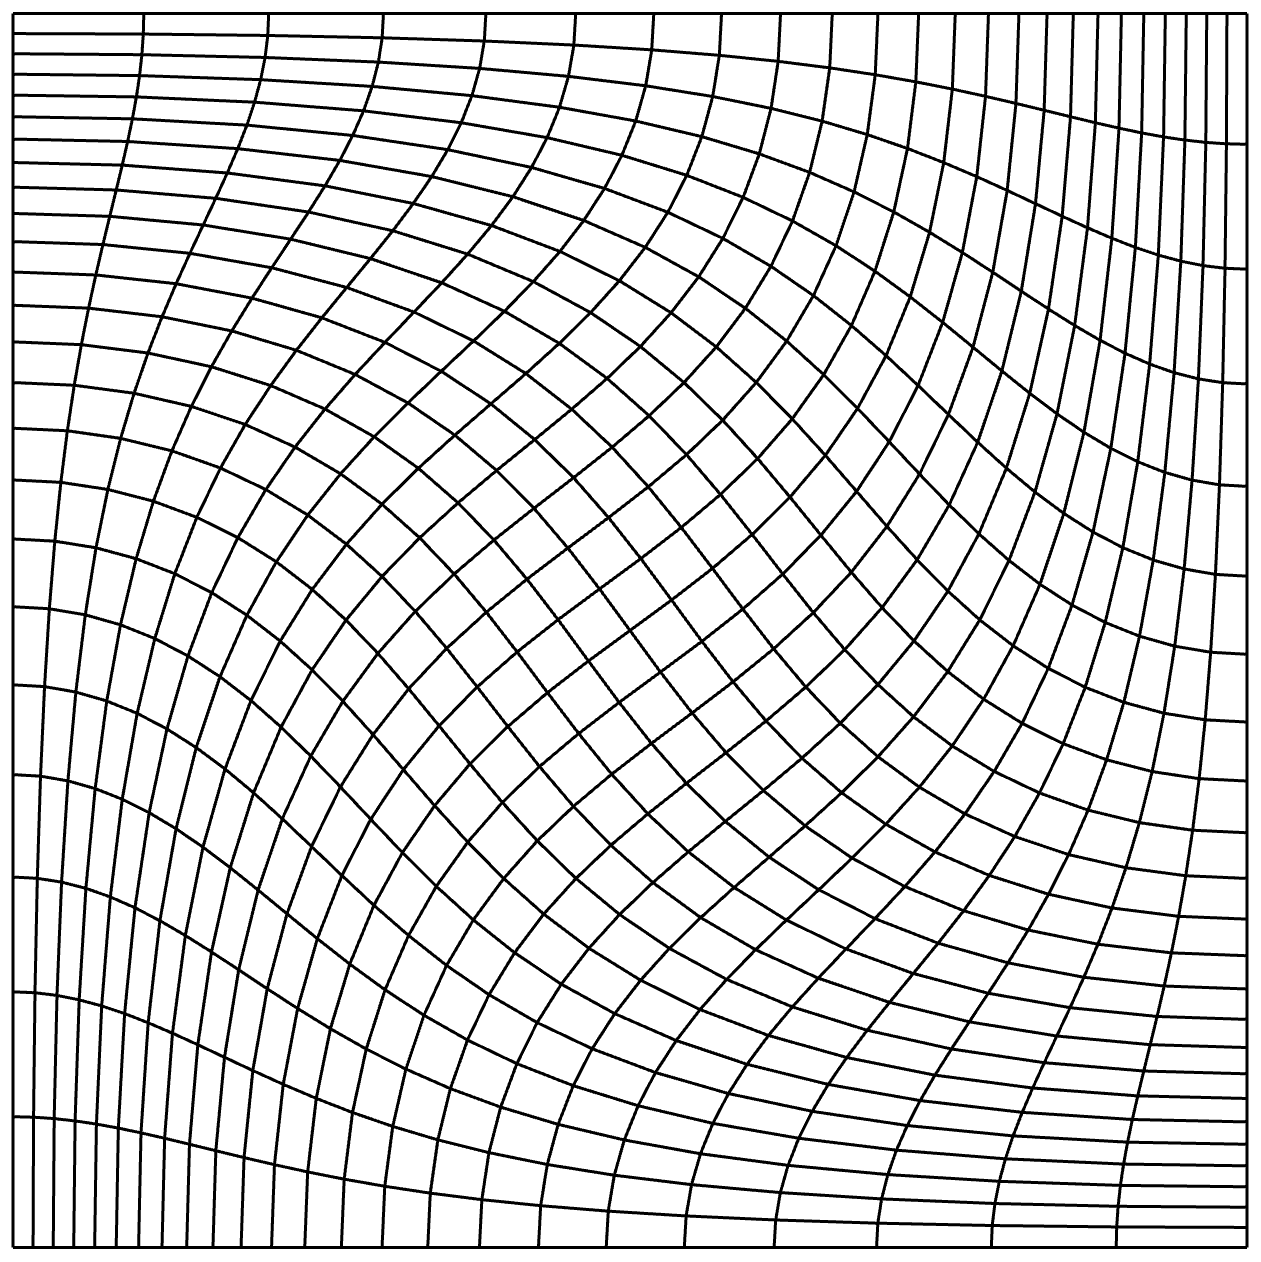
\includegraphics[width=.5\textwidth]{data/img/tgmesh0.3.png}
\caption{An example of a third-order mesh distorted by advecting the interior nodes according to the velocity field of the Taylor-Green hydrodynamics problem. }
\label{dgvef:tgmesh}
\end{figure}

Figure \ref{dgvef:mms_plot} shows the $L^2(\D)$ error between the VEF solution and the exact MMS scalar flux solution as the mesh is refined for the IP, BR2, MDLDG, and CG VEF discretizations when quadratic basis functions are used. Here, $h$ is the \emph{maximum} value of the characteristic element length in the mesh. All methods have nearly identical error behavior and converge with third-order accuracy as expected. This experiment is repeated with $p=1$ and $p=3$ in Tables \ref{dgvef:mms_table1} and \ref{dgvef:mms_table2}, respectively. Logarithmic regression is used to compute the exponent and constant of the error function $E = C h^{\bar{p}}$ with $C$ the constant and $\bar{p}$ the method's experimentally-observed order of accuracy. The standard deviation of the four error values for each value of $h$ is also provided to quantify the variance in the error behavior. Accuracy of $\mathcal{O}(h^{p+1})$ is observed and the four variants are shown to have variance below the discretization error. 

% --- MMS tables --- 
\begin{table}
\centering
\caption{MMS error for each method as a function of the \emph{maximum} characteristic mesh size, $h$. The standard deviation of the four error values in each row is also provided. First-order polynomial basis functions were used. The order of accuracy and error constant were computed with logarithmic regression. }
\label{dgvef:mms_table1}
\input{figs/dgvef/mms_table}
\end{table}

\begin{table}
\centering
\caption{MMS error for each method as a function of the \emph{maximum} characteristic mesh size, $h$. The standard deviation of the four error values in each row is also provided. Third-order polynomial basis functions were used. The order of accuracy and error constant were computed with logarithmic regression. }
\label{dgvef:mms_table2}
\input{figs/dgvef/mms_table_2}
\end{table}

% --- MMS plot --- 
\begin{figure}
\centering
\includegraphics[width=.65\textwidth]{figs/dgvef/mms_1.pdf}
\caption{The error in the scalar flux as the mesh is refined. Quadratic basis functions were used. Comparison to the reference third-order slope indicates all methods converge with optimal third-order accuracy. }
\label{dgvef:mms_plot}
\end{figure}

\subsection{Thick Diffusion Limit}
Next, we investigate the iterative convergence properties of the VEF methods in the regime known as the asymptotic thick diffusion limit \cite{diflim}. The material data are set to 
	\begin{equation}
		\sigma_t = \frac{1}{\epsilon} \,, \quad \sigma_a = \epsilon \,, \quad \sigma_s = \frac{1}{\epsilon} - \epsilon \,, \quad q = \epsilon 
	\end{equation}
with $\epsilon \in (0,1]$ and the thick diffusion limit corresponding to $\epsilon \rightarrow 0$. A coarse mesh that does not adequately resolve the mean free path is used to stress the convergence of the VEF algorithm. This is a numerically challenging, but common in practice, regime where robust performance is crucial. 

We first demonstrate robust convergence on an $8\times 8$ linear mesh with $\D = [0,1]^2$. Convergence was identical for linear, quadratic, and cubic basis functions so we present results for $p=2$ only. Level symmetric $S_4$ angular quadrature is used. Fixed-point iteration without Anderson acceleration is used to solve the coupled transport-VEF system. Table \ref{dgvef:tdl} shows the number of iterations required to converge to a fixed-point tolerance of $10^{-6}$ as $\epsilon \rightarrow 0$. All four VEF variants converge robustly and in an identical number of iterations for each value of $\epsilon$. All methods converged to the non-trivial diffusion limit solution. Lineouts of the 2D solutions are shown in Fig.~\ref{dgvef:eps_lineout} to demonstrate that the non-trivial, diffusion solution is obtained by each of the four methods. Note that even the continuous finite element discretization paired with the discontinuous finite element transport discretization was( robust in the thick diffusion limit. 
% --- thick diffusion limit --- 
\begin{table}
\centering
\caption{Number of iterations to convergence in the thick diffusion limit on a coarse, orthogonal mesh.}
\label{dgvef:tdl}
\input{figs/eps_table}
\end{table}
% --- orthogonal lineouts --- 
\begin{figure}
\centering
\foreach \f in {figs/eps_lineout.pdf,figs/eps_lineout_br2.pdf,figs/eps_lineout_mdldg.pdf,figs/eps_lineout_cg.pdf}{
	\begin{subfigure}{.4\textwidth}
	\centering
	\includegraphics[width=\textwidth]{\f}
	\caption{}
	\end{subfigure}	
}
\caption{Lineouts of the 2D thick diffusion limit solutions taken at $y=\frac{1}{2}$ for the (a) IP, (b) BR2, (c) MDLDG, and (d) CG methods.}
\label{dgvef:eps_lineout}
\end{figure}

This experiment is repeated on the triple point mesh shown in Fig.~\ref{dgvef:3point_mesh}. This mesh was generated by running a purely Lagrangian hydrodynamics simulation on a third-order mesh. The mesh contains concave/reentrant interior faces meaning the matrix corresponding to the transport discretization \emph{cannot} be re-ordered to be strictly lower block triangular. The pseudo-optimally reordered sweep from \cite{graph_sweeps}, which lags the incoming angular flux on reentrant faces, is used to enable an element-by-element transport solve. Since the incoming fluxes on reentrant faces are lagged, the angular flux on these faces is not linearly eliminated. In other words, the presence of reentrant faces means that the transport equation is not fully inverted at every fixed-point iteration. In addition, the mesh elements in the ``swirl'' at the center are severely distorted and thus have poor approximation ability. In practice, the mesh would be remapped before this level of distortion were present. Due to this severe distortion, stability of the IP VEF discretization required scaling the penalty parameter according to 
	\begin{equation}
		\kappa_e = C \frac{(p+1)^2}{\sigma_t h_e} \,,
	\end{equation}	
where $C = \max_{K_e \in \meshT} C_e$ with $C_e$ the condition number of the Jacobian matrix for element $K_e$. For the triple point mesh, $C=169$.
% --- triple point mesh --- 
\begin{figure}
\centering
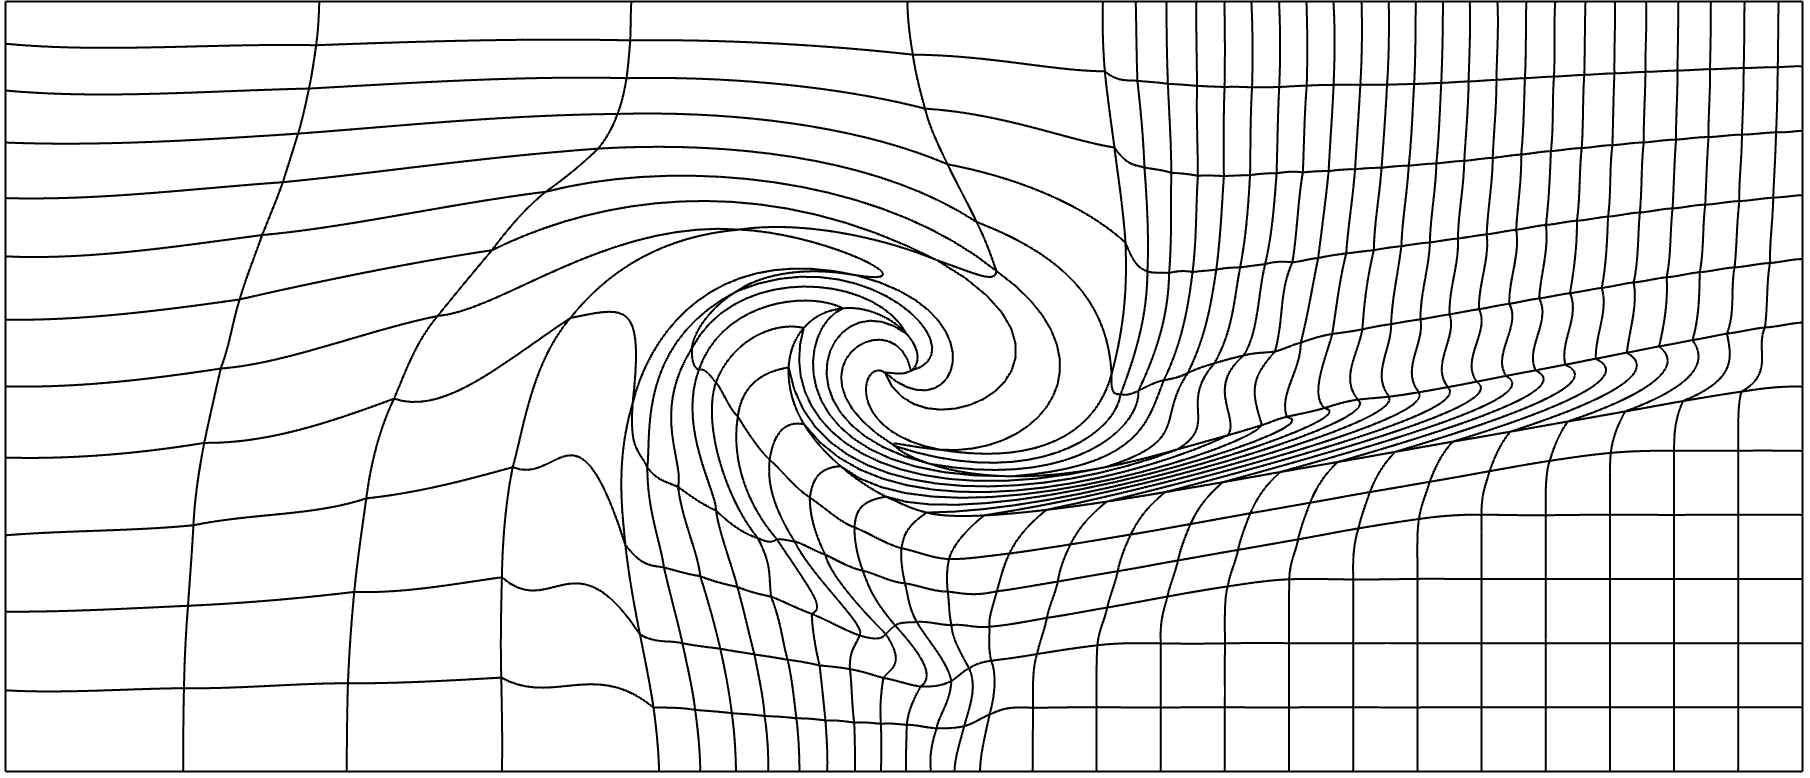
\includegraphics[width=.65\textwidth]{data/img/3point.png}
\caption{A depiction of the triple point mesh used to stress test the VEF algorithms on a severely distorted, third-order mesh. The mesh was generated with a purely Lagrangian hydrodynamics simulation. }
\label{dgvef:3point_mesh}
\end{figure}

Table \ref{dgvef:tdl_3p} shows the number of fixed-point iterations to converge the thick diffusion limit problems on the triple point mesh. The IP, BR2, and CG methods converged equivalently with MDLDG generally converging slower. This is likely due to MDLDG being less numerically diffusive compared to the IP, BR2, and CG methods which either have a penalization term that regularizes towards a continuous solution or is a continuous method. 
% --- triple point TDL --- 
\begin{table}
\centering
\caption{Number of fixed-point iterations required for convergence on the triple point mesh as $\epsilon \rightarrow 0$. On the triple point mesh, reentrant faces mean the transport equation is not fully inverted at each iteration.}
\label{dgvef:tdl_3p}
\input{figs/eps_table_dgvef_3p}
\end{table}

\subsection{Crooked Pipe} \label{dgvef_sec:cp}
We now demonstrate the efficacy of the methods on a more realistic, multi-material problem. A common benchmark is the crooked pipe problem. The geometry and materials are shown in Fig.~\ref{dgvef:cp_diag}. The problem consists of two materials, the wall and the pipe, which have an 1000x difference in total interaction cross section. We mock the time-dependent benchmark as a steady-state problem by adding artificial absorption and fixed-source terms corresponding to backward Euler time integration. We use a large time step such that $c\Delta t = 10^3$ with an initial condition $\psi_0 = 10^{-4}$ for all $(\x,\Omegahat) \in \D \times \mathbb{S}^2$. The absorption and source terms are then 
	\begin{subequations}
	\begin{equation}
		\sigma_a = \frac{1}{c\Delta t} = 10^{-3} \,\si{\per\cm}\,,  
	\end{equation}
	\begin{equation}
		q = \frac{1}{c\Delta t} \psi_0 = 10^{-1}\,\si{\per\cm\cubed\per\s\per\str} \,. 
	\end{equation}
	\end{subequations}
The boundary conditions are 
	\begin{equation}
		f = \begin{cases}
			\frac{1}{2\pi}\,, & x = 0 \ \mathrm{and}\ y \in [-1/2,1/2] \\ 
			0 \,, & \mathrm{otherwise}
		\end{cases} \,,
	\end{equation}
so that radiation enters the pipe at the left side of the domain. We use a Level Symmetric $S_{12}$ angular quadrature set. The zero and scale \cite{hamilton2009negative} negative flux fixup, a sweep compatible method that zeros out negativity and rescales so that particle balance is preserved, is used inside the transport inversion to ensure positivity. 
% --- crooked pipe geometry --- 
\begin{figure}
\centering
\includegraphics[width=.65\textwidth]{figs/crooked_pipe.pdf}
\caption{Geometry, material data, and boundary conditions for the linearized crooked pipe problem.}
\label{dgvef:cp_diag}
\end{figure}

A VEF solution to the crooked pipe using the IP method with $p=2$ is shown in Fig.~\ref{dgvef:cp_sol} where a non-uniform mesh is used to adequately resolve the interface between the optically thin pipe and the optically thick wall. Here, we see that VEF does capture the ``shadow'' induced by the radiation turning the corner around the inner wall. A radiation diffusion solution would non-physically show illumination on the back side of the wall.
% --- crooked pipe solution --- 
\begin{figure}
\centering
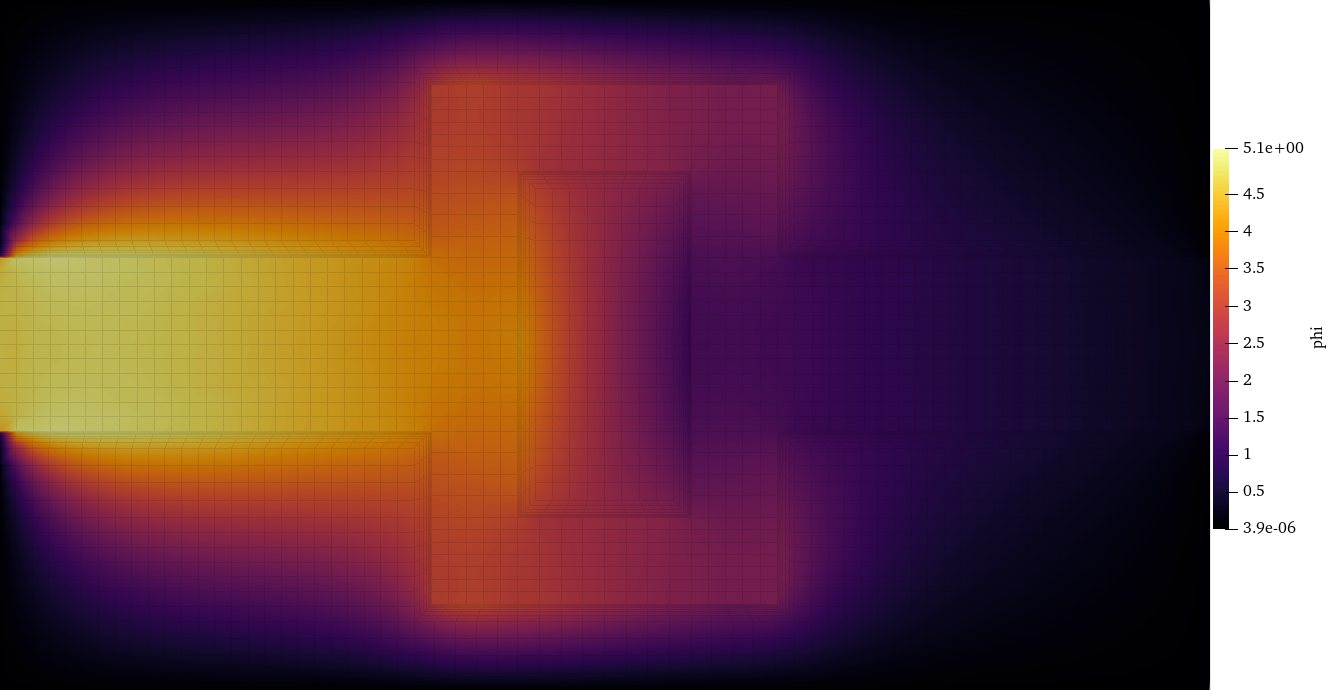
\includegraphics[width=.65\textwidth]{data/img/cp.png}
\caption{VEF scalar flux solution to the linearized crooked pipe problem to show that VEF does capture the transport solution. The mesh is refined at the interface between thick and thin to adequately resolve the material interface. The IP VEF method with $p=2$ was used.}
\label{dgvef:cp_sol}
\end{figure}

The outer fixed-point and inner linear iterative efficiency is demonstrated by refining in $h$ and $p$. Note that to simplify the refinement process we use a uniform mesh. The outer solver is Anderson-accelerated fixed-point iteration with two Anderson vectors. Anderson acceleration is not required for convergence on this problem but does provide more uniform convergence in $h$. Since the mesh is orthogonal, the transport equation is fully inverted at each outer iteration. This allows use of the low memory variant so that the storage cost of Anderson acceleration is two scalar flux-sized vectors. The outer tolerance is $10^{-6}$. The inner \gls{bicg} tolerance is $10^{-8}$. The \gls{usc} preconditioner with one Jacobi iteration and one \gls{amg} V-cycle per application is used for the IP and BR2 discretizations. The CG and MDLDG discretizations use one V-cycle of AMG as a preconditioner. The previous outer iteration is used as an initial guess to \gls{bicg} so that the initial guess becomes progressively better as the outer iteration converges. 

Table \ref{dgvef:cphp} shows the number of outer Anderson-accelerated fixed-point iterations and the maximum, minimum, and average number of inner \gls{bicg} iterations performed at each outer iteration as the mesh is refined and the polynomial order is increased. At each refinement and polynomial order, the IP, BR2, and CG methods outer iteration converged equivalently with MDLDG converging 1-4 iterations slower. All methods were scalable in $h$ and $p$ with CG requiring the fewest iterations followed by MDLDG and then IP and BR2. 
% --- crooked pipe hp scaling --- 
\begin{table}
\centering
\caption{The number of Anderson-accelerated fixed-point iterations until convergence to a tolerance of $10^{-6}$ for the IP, BR2, MDLDG, and CG discretizations of VEF on the linearized crooked pipe problem refined in $h$ and $p$. An Anderson space of size two is used.}
\label{dgvef:cphp}
\begin{adjustbox}{max width = \textwidth}
\input{figs/cp_dgvef.tex}
\end{adjustbox}
\end{table}

\subsection{Weak Scaling} \label{dgvef_sec:weak}
Finally, we show that the IP and CG VEF system with $p=2$ can be solved efficiently in parallel on larger problems. The parallel partitioning is such that there are $\sim\!9000$ VEF scalar flux unknowns per processor. The results were generated on 32 nodes of the \texttt{rztopaz} machine at LLNL which has two 18-core Intel Xeon E5-2695 CPUs per node. 

First, we investigate weak scaling on a mock problem where the VEF data are provided as inputs to the problem (as opposed to being solved for through fixed-point iteration). This allows the VEF system to be solved in isolation from the transport equation. We use the materials, geometry, and boundary conditions from the crooked pipe problem shown in Fig.~\ref{dgvef:cp_diag} but set the Eddington tensor and boundary factor to 
	\begin{subequations}
	\begin{equation}
		\E = \begin{cases}
			\begin{bmatrix} 
				9/11 & 0 \\ 0 & 1/11 
			\end{bmatrix}\,, & \x \in \mathrm{pipe} \\[1em] 
			\begin{bmatrix} 
				1/3	& 0 \\ 0 & 1/3
			\end{bmatrix}\,, & \x \in \mathrm{wall} 
		\end{cases} \,, 
	\end{equation}
	\begin{equation}
		E_b = \begin{cases}
			9/10 \,, & \x \in \partial(\mathrm{pipe})\\
			1/2 \,, & \x \in \partial(\mathrm{wall}) 
		\end{cases} \,. 
	\end{equation}
	\end{subequations}
This corresponds to a linearly-anisotropic/diffusive angular flux in the wall and an extremely forward peaked solution 
	\begin{equation}
		\psi = \Omegahat_x^8 
	\end{equation}
in the pipe. The motivation for this choice is that the solvers are predicted to struggle when the Eddington tensor is discontinuous. We stress that this setup does not correspond to a physically realistic problem. 

Table \ref{dgvef:weak_mock} shows the number of \gls{bicg} iterations to convergence for the USC-preconditioned IP VEF system on this mock problem. The columns of the table parameterize the solver used for the continuous stage of the USC preconditioner. The standard USC preconditioner used in the previous results did not converge on this mock problem. However, when a sparse direct solver is used instead of AMG, uniform convergence is recovered. This suggests that AMG is failing to adequately solve the continuous operator. 
% --- weak scaling mock problem --- 
\begin{table}
\centering
\caption{Weak scaling the IP VEF method with $p=2$ on a non-physically difficult problem with mock VEF data. The preconditioner is parameterized by the method used for the approximate inverse of the continuous operator. The standard USC preconditioner with AMG on the continuous operator did not converge due to the large discontinuity in the VEF data. Convergence is recovered by applying AMG to a symmetrized version of the CG operator.}
\label{dgvef:weak_mock}
\input{figs/dgvef/mock}
\end{table}

Note that AMG is effective on the standard continuous finite element discretization of diffusion. It is then expected that AMG will be effective in approximating the inverse of a symmetrized CG operator. By lagging the terms 
	\begin{equation}
		-\int_{\Gamma_0} \avg{\frac{\nabla u}{\sigma_t}}\cdot \jump{\E\varphi\n} \ud s + \int \nabla u \cdot \frac{1}{\sigma_t} \paren{\nablah\cdot\E}\!\varphi \ud \x
	\end{equation}
in the CG VEF discretization (Eq.~\ref{dgvef:cg}), a symmetric operator more amenable to accurate inversion via AMG is found. The symmetrized operator is then:
	\begin{equation}
		\int_{\Gamma_b} E_b\, u \varphi \ud s + \int \nablah u \cdot \frac{1}{\sigma_t}\E \nablah \varphi \ud \x + \int \sigma_a\, u \varphi \ud \x \,, 
	\end{equation}
with $u,v \in V_p$. 
This is a CG discretization of 
	\begin{equation}
		-\nabla \cdot \frac{1}{\sigma_t}\E\nabla \varphi + \sigma_a \varphi 
	\end{equation} 
which corresponds to the VEF drift-diffusion equation where the advective term $\paren{\nabla\cdot\E}\!\varphi$ is lagged and moved to the right hand side. 

The ``AMG-S'' column of Table \ref{dgvef:weak_mock} shows the convergence on the mock problem when one AMG V-cycle is applied to the symmetrized CG operator instead of the non-symmetric CG operator. The method converges and is roughly uniform in iteration counts as the mesh is refined. The ``AMG-S3'' column corresponds to the use of three iterations of an inner Richardson iteration to approximate the inverse of the non-symmetric CG operator. The Richardson iteration is preconditioned using one V-cycle of AMG on the symmetrized CG operator. In other words, this option approximates the inverse of the non-symmetric CG operator with three approximate inversions of the symmetrized CG operator. For this option, iterative efficiency generally fell between that of the sparse direct solver and using only AMG on the symmetrized CG operator. Inner iterations do reduce the number of total iterations to convergence but, since three V-cycles are performed per preconditioner application, not to the degree that fewer V-cycles are performed.

Next, we show weak scaling of the IP and CG VEF linear solves on the first outer iteration of the linearized crooked pipe problem from Section \ref{dgvef_sec:cp} with $p=2$. One parallel block Jacobi transport sweep is performed to provide angular fluxes to compute the VEF data. The VEF system is then solved using \gls{bicg}. Table \ref{dgvef:weak_cp} shows the number of \gls{bicg} iterations to convergence to a tolerance of $10^{-8}$. For the IP method, the USC preconditioner is used where the continuous operator is left in non-symmetric form and when it is symmetrized. The CG method uses AMG as a preconditioner. In addition, the number of iterations to solve the corresponding IP and CG diffusion problems (by setting $\E = \frac{1}{3}\I$ and $E_b = 1/2$) are shown. These results indicate that on a physically realistic problem the standard USC preconditioner and USC preconditioner with the symmetrized CG operator are both effective. IP VEF only required 5-7 more iterations than IP diffusion and CG VEF only required 2-7 more iterations than CG diffusion. Since no problems where the USC preconditioner with symmetrized CG operator failed to converge were found, the preconditioner with symmetrized CG operator may be more robust. Note that this discrepancy was not observed on physically realistic problems. 
% --- weak scaling on cp --- 
\begin{table}
\centering
\caption{Weak scaling the IP and CG VEF methods with $p=2$ on the first iteration of the linearized crooked pipe problem. A parallel block Jacobi sweep was used to generate the VEF data needed to form the VEF system. On this physically realistic problem, both the standard USC and USC with symmetrized CG operator converged uniformly. The iterative efficiency is compared to solving the corresponding IP and CG radiation diffusion problems. }
\label{dgvef:weak_cp}
\input{figs/dgvef/weak}
\end{table}

\end{document}